\documentclass[20pt,a0paper,landscape]{tikzposter}

%% Tikzposter is highly customizable: please see
%% https://bitbucket.org/surmann/tikzposter/downloads/styleguide.pdf

%% Available themes: see also
%% https://bitbucket.org/surmann/tikzposter/downloads/themes.pdf
% \usetheme{Default}
% \usetheme{Rays}
%\usetheme{Basic}
%\usetheme{Simple}
 \usetheme{Envelope}
% \usetheme{Wave}
% \usetheme{Board}
% \usetheme{Autumn}
% \usetheme{Desert}

%% Further changes to the title etc is possible
% \usetitlestyle{Default}
% \usetitlestyle{Basic}
% \usetitlestyle{Empty}
% \usetitlestyle{Filled}
% \usetitlestyle{Envelope}
% \usetitlestyle{Wave}
 %\usetitlestyle{verticalShading}

\definecolor{dukeblue}{HTML}{00539B}

\colorlet{backgroundcolor}{white}
\colorlet{blocktitlebgcolor}{dukeblue}
\colorlet{blocktitlefgcolor}{white}
\colorlet{blockbodybgcolor}{white}
\colorlet{blockbodyfgcolor}{black}

\usepackage{fontspec}
\setmainfont{FreeSerif}
\setsansfont{FreeSans}

\author{Vinay Tripuraneni\textsuperscript{1}, Gonen Memisoglu\textsuperscript{2}, Wei Zhu\textsuperscript{1}, James E Haber\textsuperscript{2}, and David M MacAlpine\textsuperscript{1}}

\title{\begin{minipage}{\textwidth}
   \centering
   Local nucleosome dynamics and eviction following a double-strand break\\ 
   \mbox{are reversible by NHEJ-mediated repair in the absence of DNA replication}
  \vspace{0.5em}\end{minipage}}

\institute{Duke University Medical Center\textsuperscript{1}, Brandeis University\textsuperscript{2}}
%% Optional title graphic
% \titlegraphic{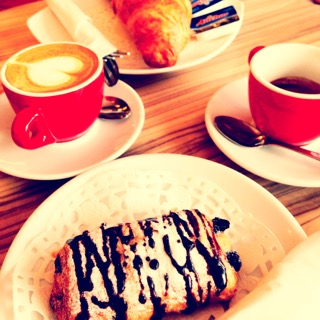
\includegraphics[width=7cm]{IMG_1934}}
%% Uncomment to switch off tikzposter footer
% \tikzposterlatexaffectionproofoff

\begin{document}
\maketitle

\begin{columns}

\column{0.25}

\block{Introduction}{
We sought to interrogate, at nucleotide-resolution, the spatiotemporal kinetics of chromatin remodeling and eviction in response to a single double strand break (DSB) and the subsequent restoration of chromatin organization following replication-independent NHEJ mediated repair. We engineered an inducible site-specific DSB system in \textit{S. cerevisiae} by inserting the 117bp HO endonuclease cut site upstream of the \textit{PHO5} locus. The \textit{PHO5} gene in yeast is marked by a well positioned +1 nucleosome that is responsible for regulating its expression and has been frequently used as a model for well defined chromatin organization. We found that local nucleosome eviction and repositioning immediately around the DSB at \textit{PHO5} occurs prior to the broad pattern of  nucleosome eviction associated with a persistent DSB. We also observed that a single nucleosome eviction event immediately adjacent to the DSB was partially dependent on \textit{MRE11} suggesting that the local end binding of MRX at a DSB may itself induce early chromatin changes at a DSB (Zhang et al. 2007). Following NHEJ- mediated repair of this break at \textit{PHO5}, we observed that the MNase sensitivity of chromatin was attenuated and that local chromatin architecture was restored rapidly. This replication- independent reassembly yields positioning of nucleosomes around the DSB that recapitulates the chromatin state prior to DSB induction suggesting that an active and structurally accurate mechanism exists to preserve chromatin architecture following DNA damage and repair.
\begin{tikzfigure}[Schematic of a DSB in the context of chromatin.  Histone octamers are evicted from the sequences surrounding the break in a \textit{MRE11}-dependent manner to facilitate repair of the DNA.  (Tsukuda et al., Nature, 2005)]
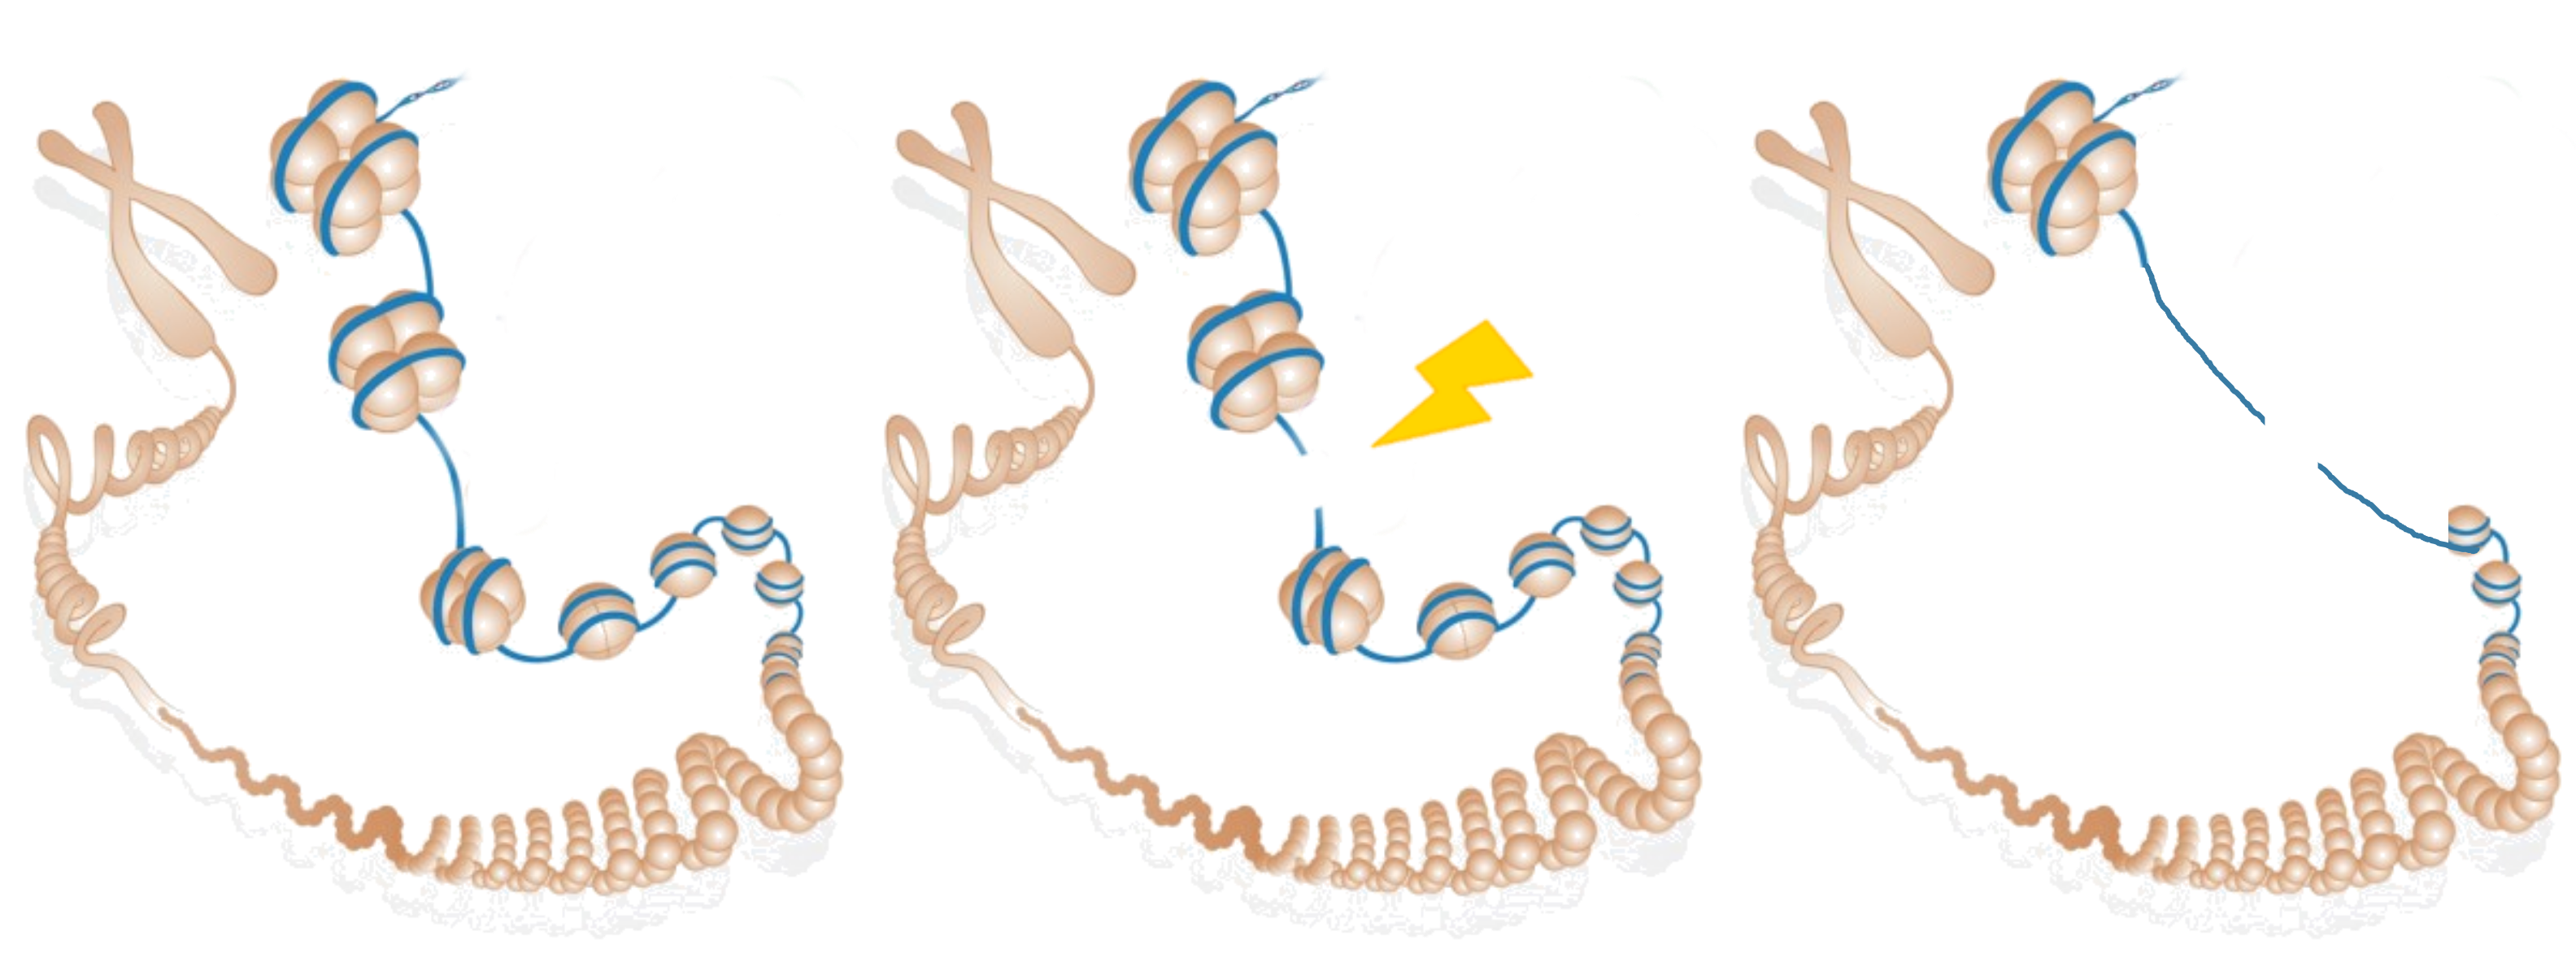
\includegraphics[width=\linewidth]{chromatin_model_dsb_eviction.png}
\end{tikzfigure}
}
\block{Inducible site-specific break at \textit{PHO5} }{
\begin{tikzfigure}[Inducible site-specific break at \textit{PHO5}.  GAL-HO induces rapid cutting at \textit{PHO5} which results in a \textit{MRE11}-dependent increase in chromatin accessibility.]
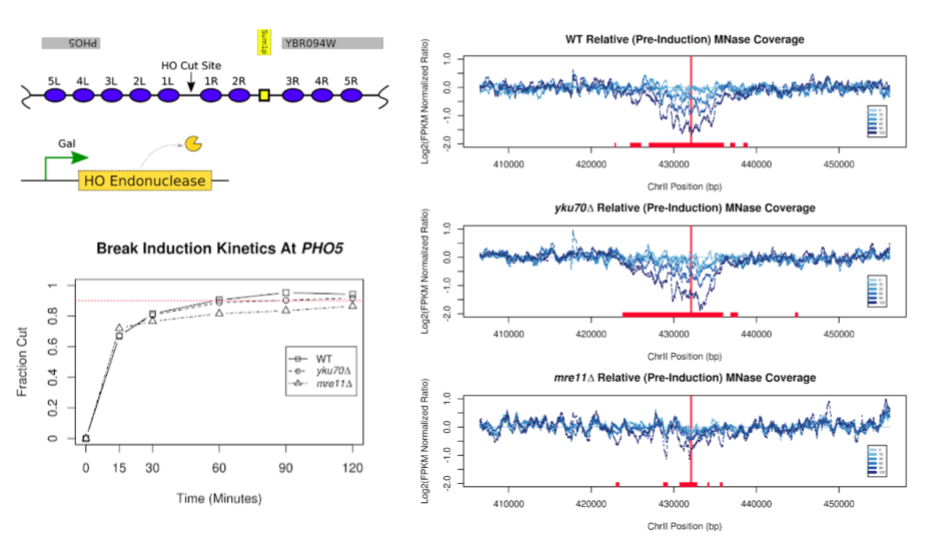
\includegraphics[width=\linewidth]{pho5_schematic_access.png}
\end{tikzfigure}
}

%\note[rotate=8, connection, width = 7cm,
% roundedcorners=15, targetoffsetx=2cm
%]{Oh wait! A note!}

%\begin{subcolumns} %\subcolumn{.5} \block{}{
%\begin{tikzfigure}[Site %specific DSB at PHO5]
%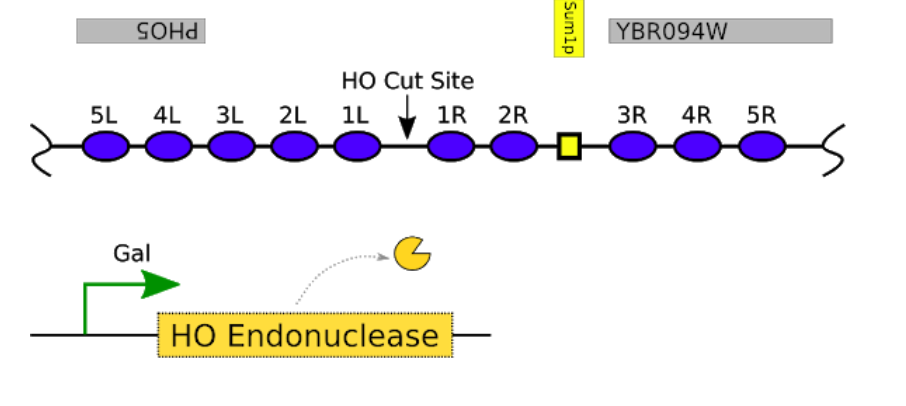
\includegraphics[width=\linewidth]{schematic.png}
%\end{tikzfigure}

%} \subcolumn{.5} \block{}{
%\begin{tikzfigure}[Cutting %efficiency at PHO5]
\%includegraphics[width=\linewi%dth]{cutting.png}
%\end{tikzfigure}
%
%} \end{subcolumns}



\column{0.25}


\block{Chromatin occupancy profiling}{%
\begin{tikzfigure}[Genome-wide chromatin occupancy profile (GCOP). Schematic of MNase based assay to generate GCOPs.  Control GCOPs for \textit{CTH1} and \textit{GAL7}.  \textit{GAL7} chromatin becomes disorganized upon galactose induction.  Pictographs summarizing changes in nucleosome positioning, occupancy and fuzziness. ]
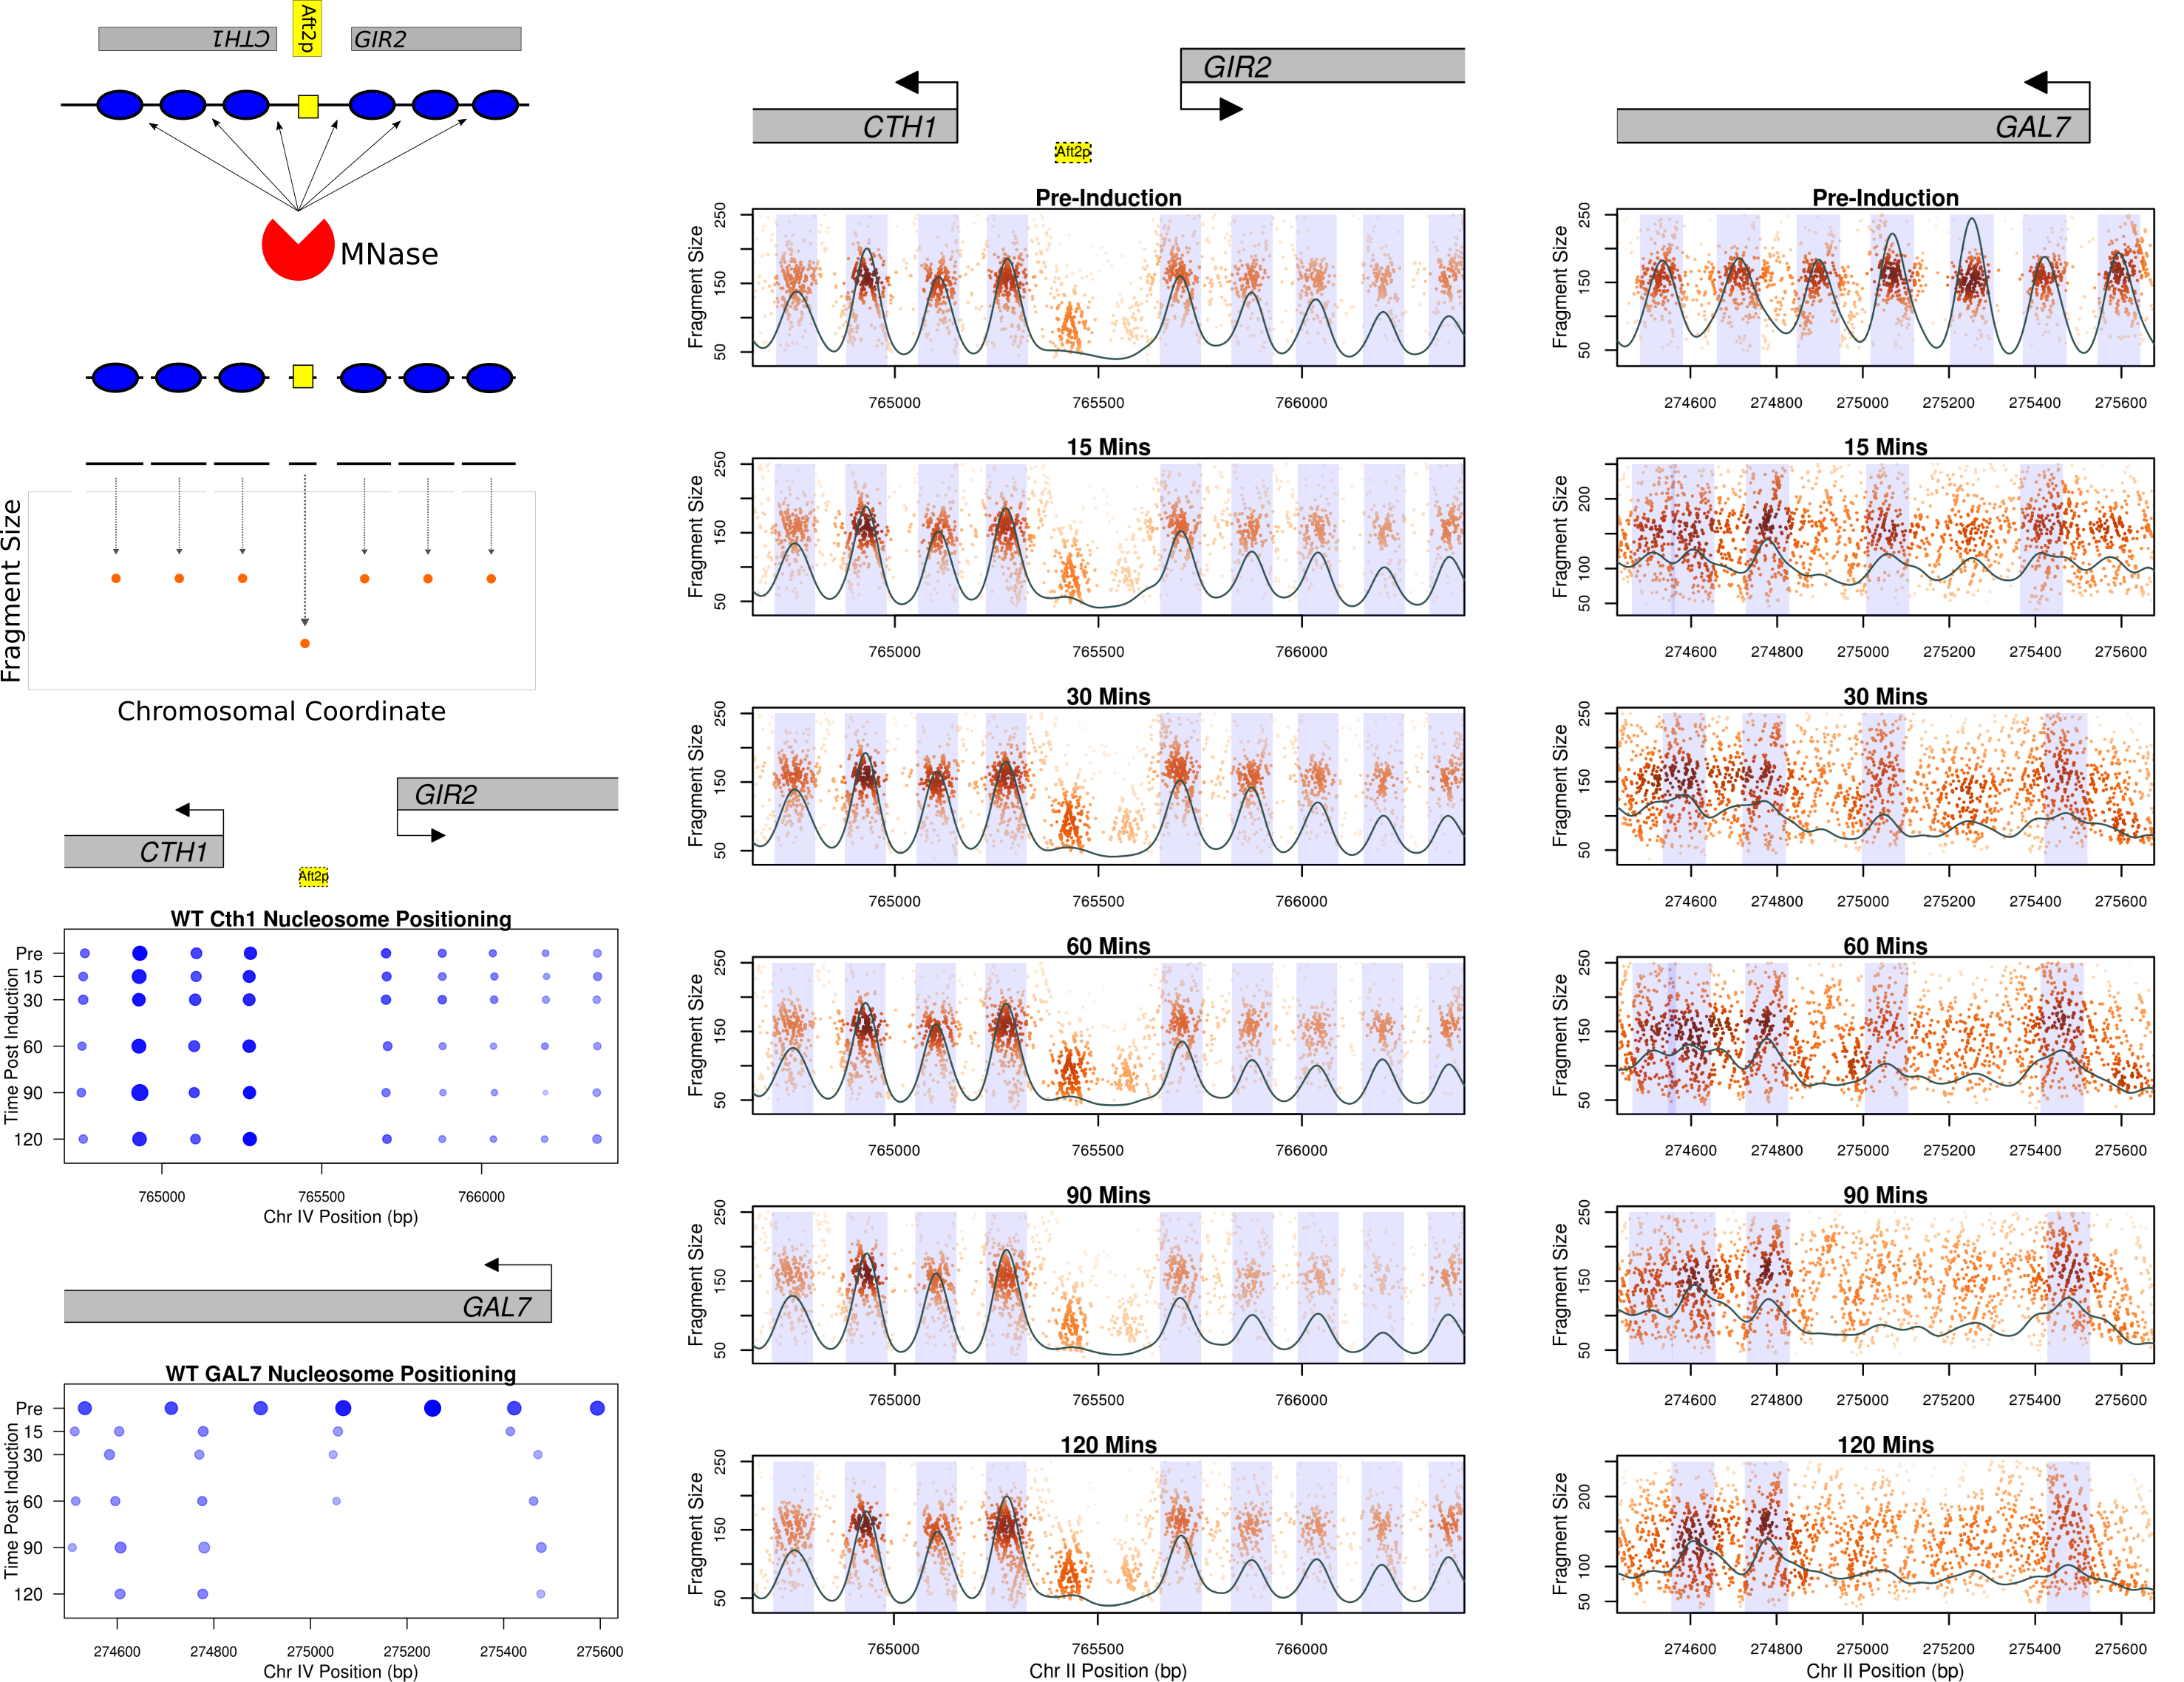
\includegraphics[width=\linewidth]{figure2_dm.png}
\end{tikzfigure}
}


\block{Chromatin occupancy profiling a DSB at the  \textit{PHO5} locus}{
\begin{tikzfigure}[Chromatin occupancy profiling at \textit{PHO5} following induction of a site specific DSB.  GCOPs are presented for WT, \textit{yku70} and \textit{mre11}.]
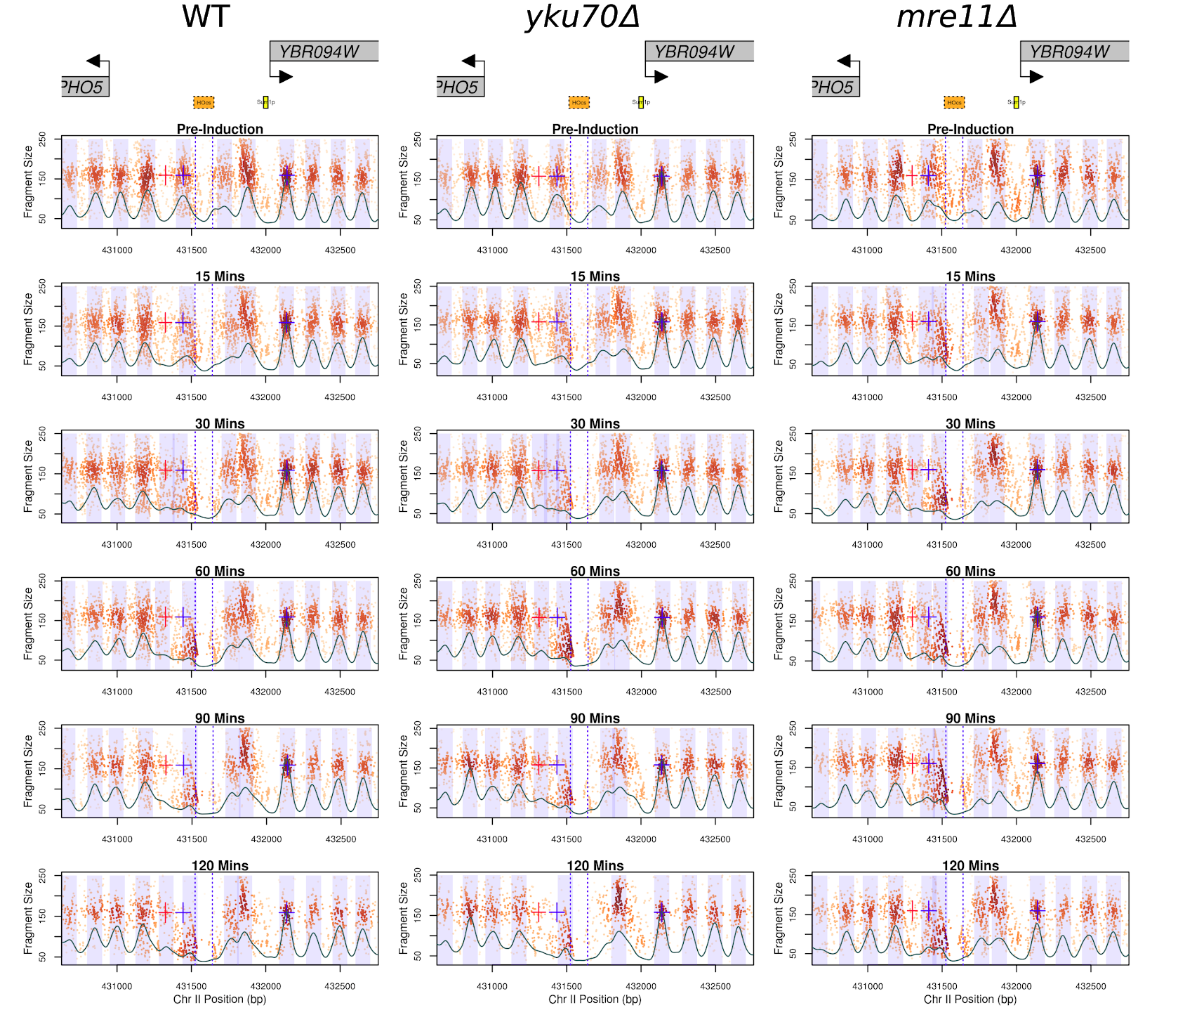
\includegraphics[width=\linewidth]{pho5_wt_mutants.png}
\end{tikzfigure}
}


\column{0.25}


\block{Histone eviction kinetics following a DSB at the  \textit{PHO5} locus}{
\begin{tikzfigure}[Histone octamer eviction kinetics at \textit{PHO5} in response to a DSB. Pictographs summarizing changes in nucleosome positioning, occupancy and fuzziness.  ]
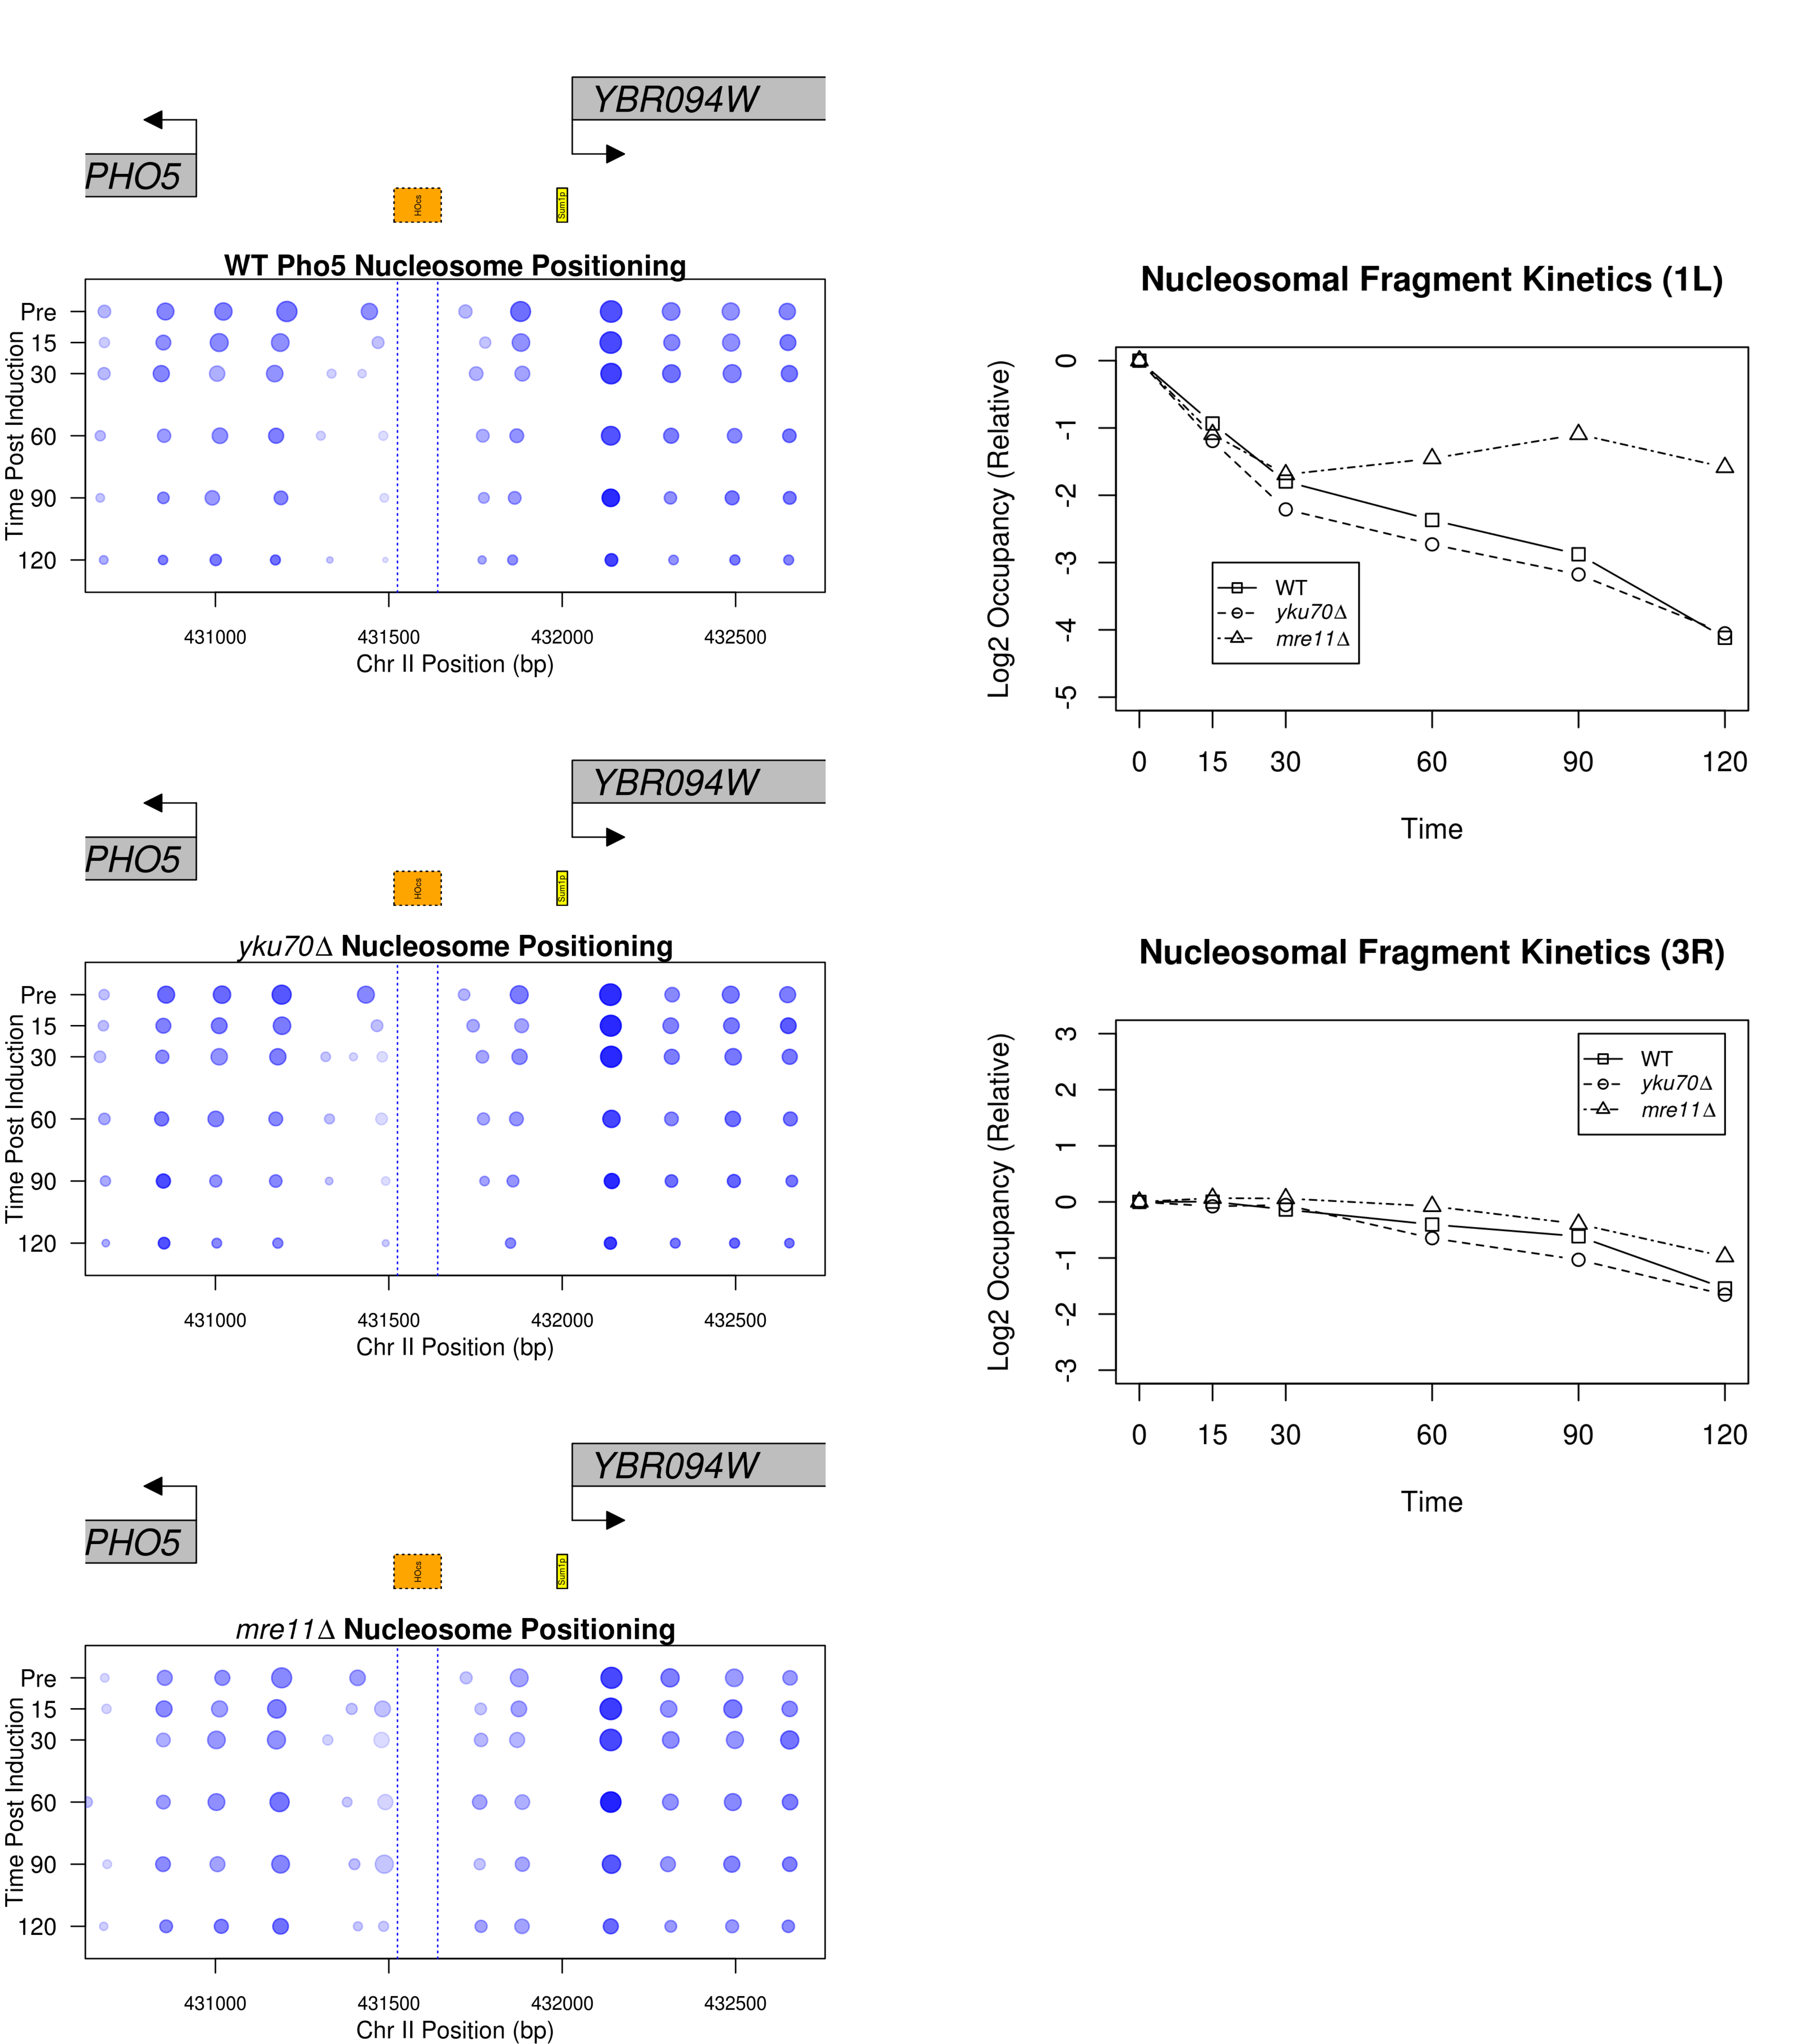
\includegraphics[width=.8\linewidth]{ho_pho5_cshl_poster.png}
\end{tikzfigure}
}

\block{Local chromatin changes in response to a DSB}{
\begin{tikzfigure}[Summary of the local and rapid chromatin changes in response to a DSB at \textit{PHO5}.  Following NHEJ repair of the break, is the epigenetic state restored in a replication-dependent or independent manner? ]
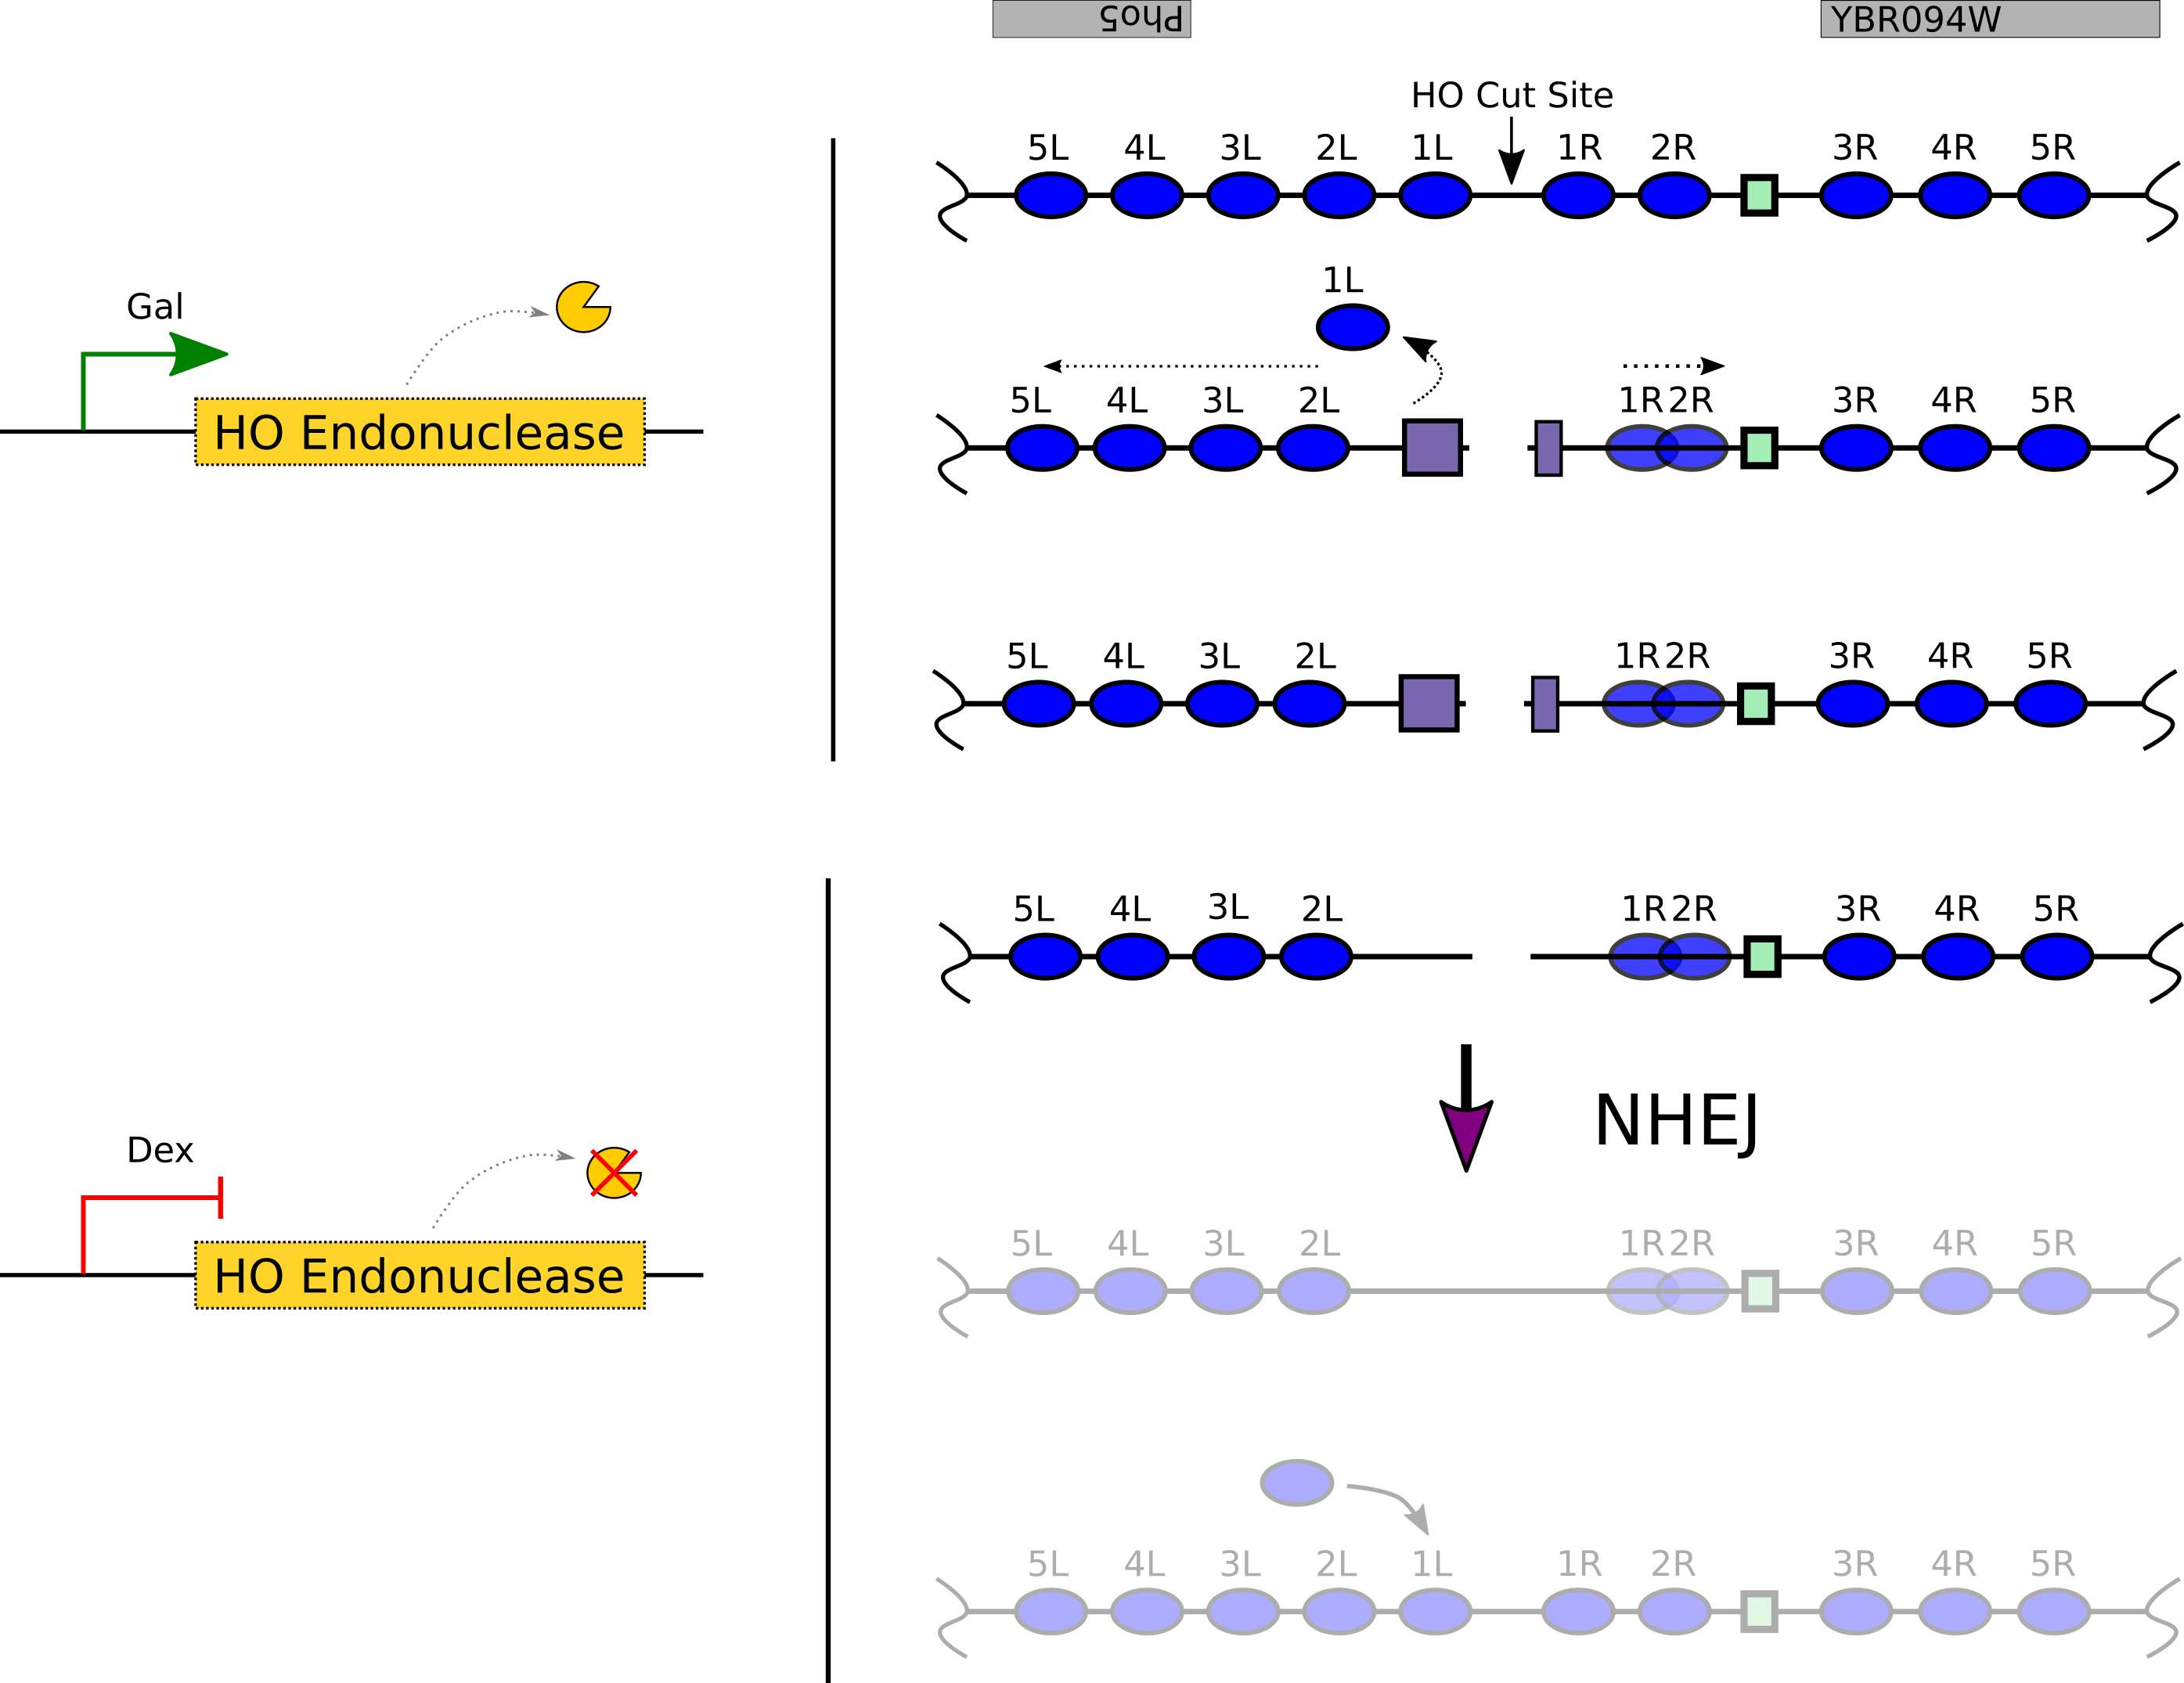
\includegraphics[width=\linewidth]{ho_nhej_model.png}
\end{tikzfigure}
}


\column{0.25}
\block{NHEJ}{
\begin{tikzfigure}[Summary of NHEJ repair following induction of a DSB at \textit{PHO5}. HR is limited by performing the experiment in a haploid strain arrested in G1 by $\alpha$-factor.]
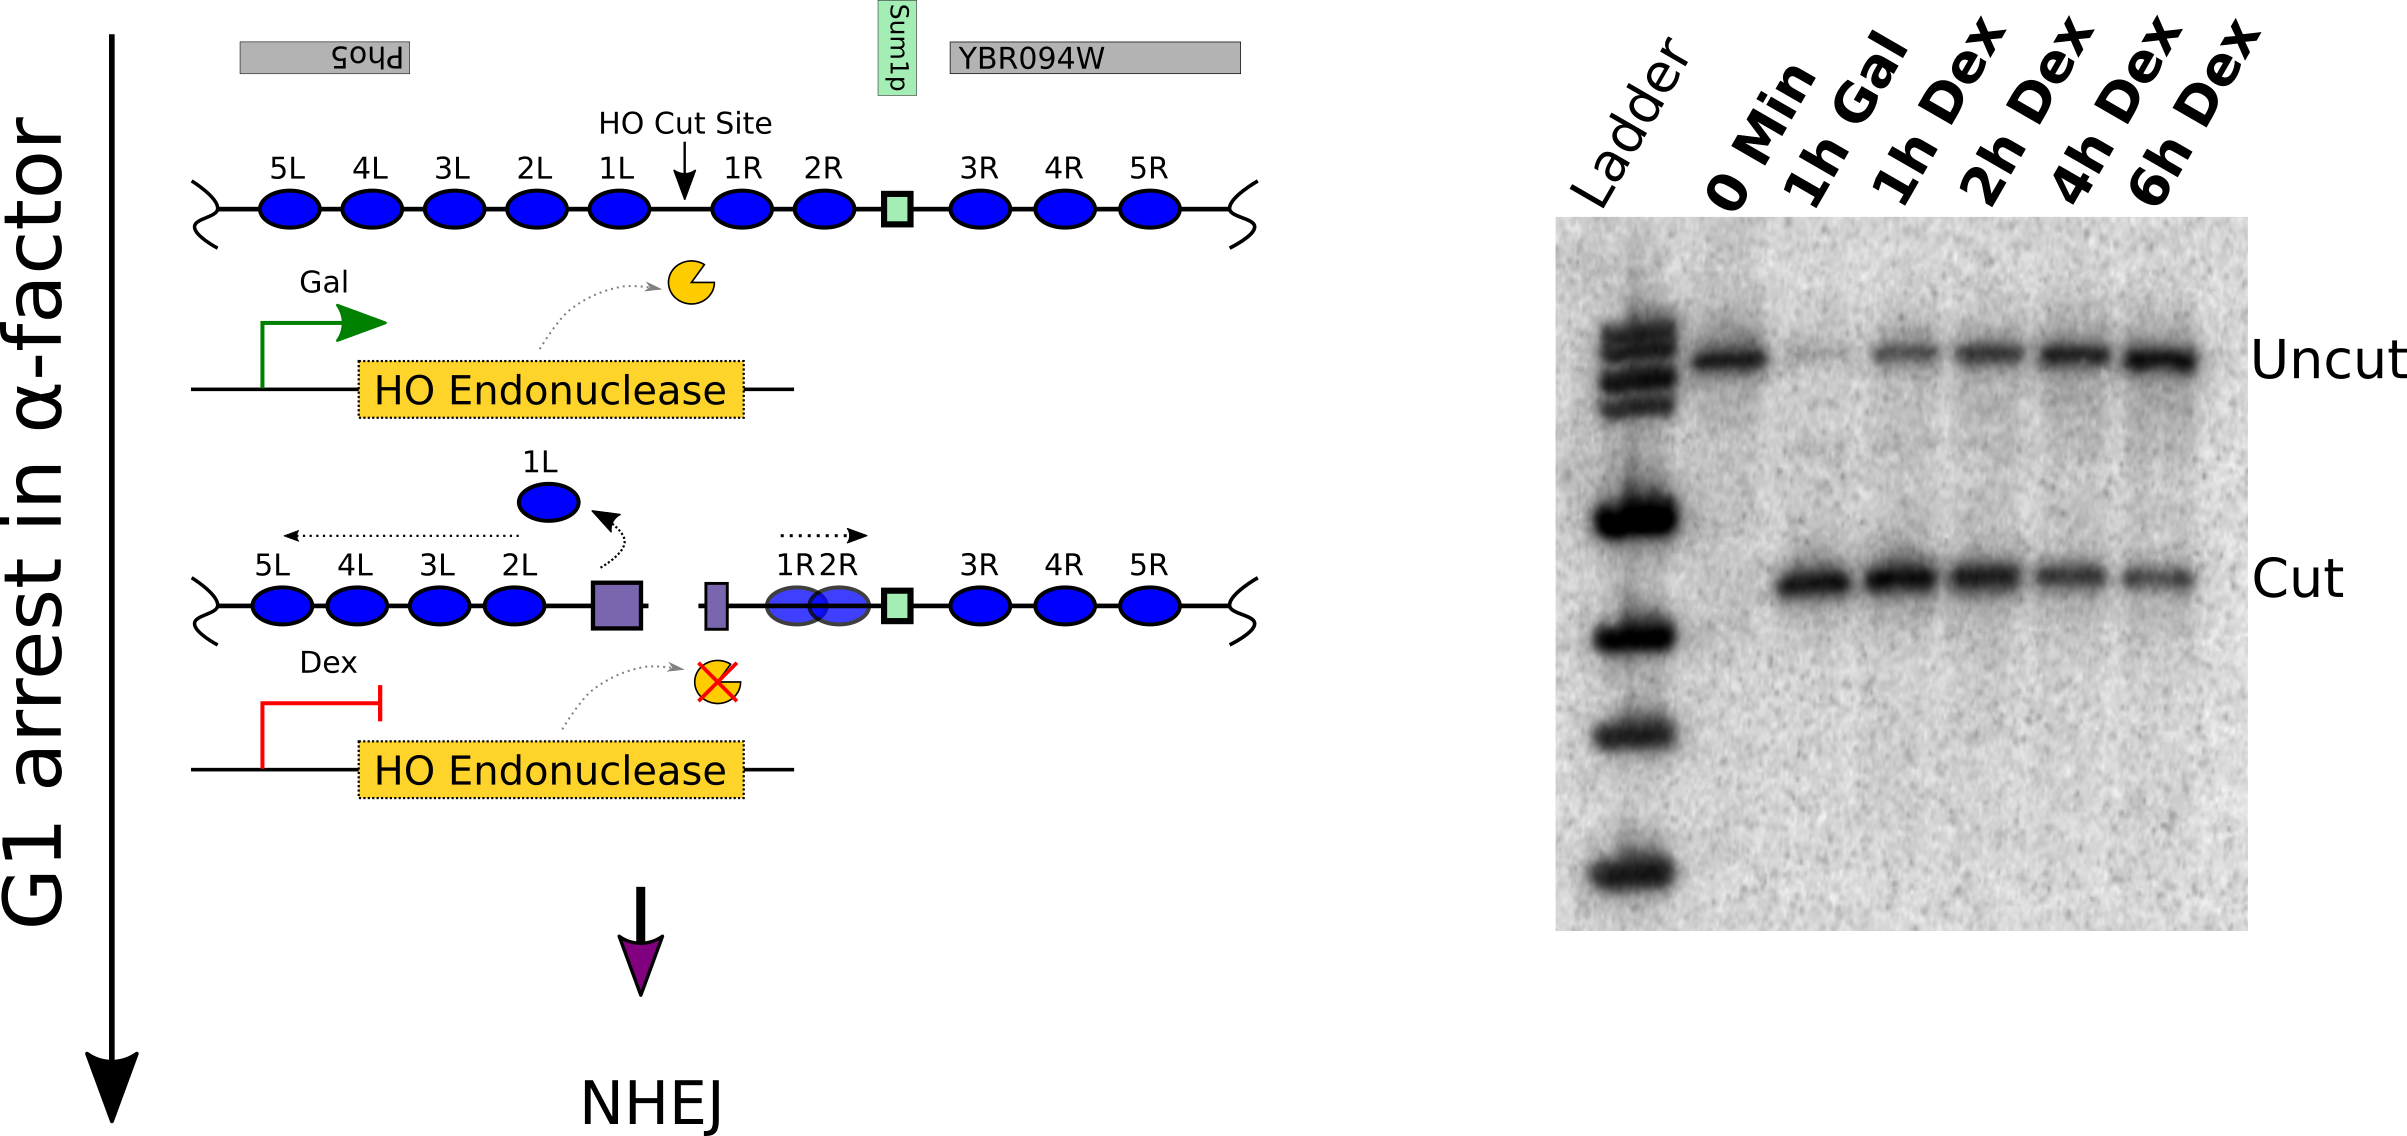
\includegraphics[width=\linewidth]{nhej_southern_model_alpha.png}
\end{tikzfigure}
}
\block{Replication-independent restoration of chromatin}{
\begin{tikzfigure}[Chromatin occupancy profiles of the \textit{PHO5} locus during NHEJ repair.  Chromatin structure is restored in a replication-independent manner.]
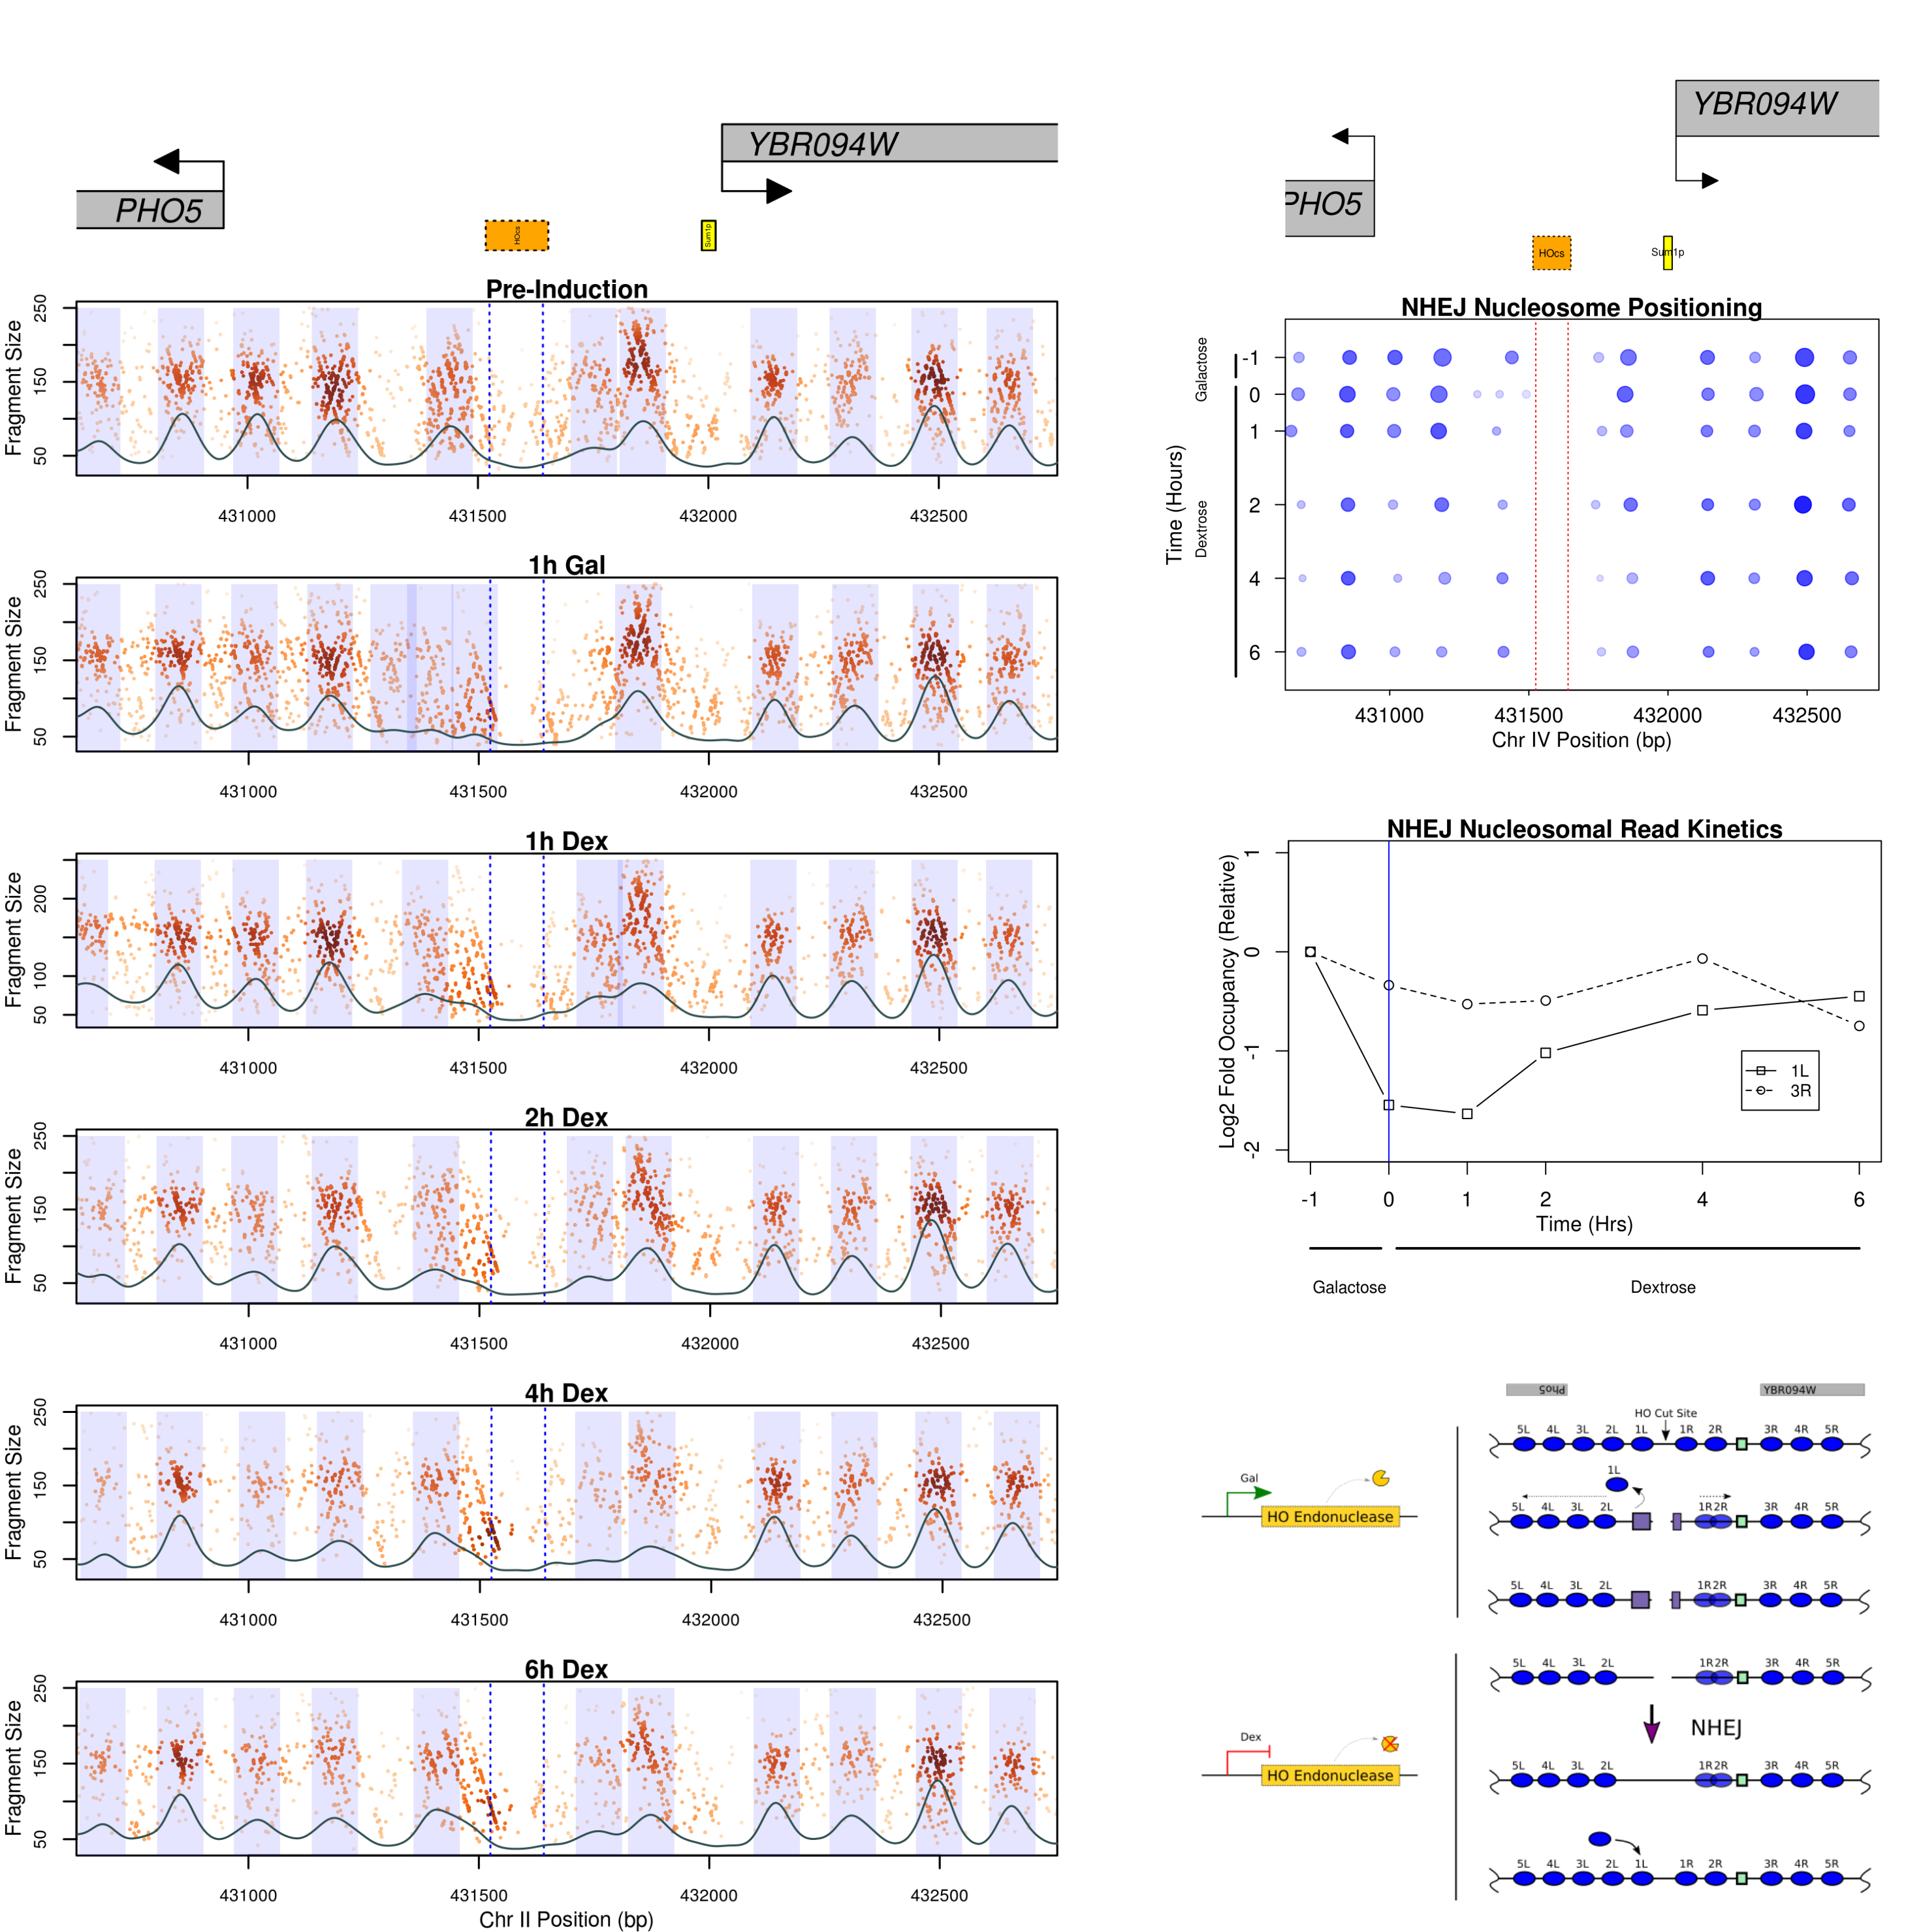
\includegraphics[width=\linewidth]{nhej_gcop_summary_2.png}
\end{tikzfigure}
}

\end{columns}



\end{document}